\documentclass[12pt]{article}

\usepackage[bottom = 15mm]{geometry}
\usepackage[utf8]{inputenc}
\usepackage[T2A]{fontenc}
\usepackage[russian]{babel}
\usepackage{graphicx}
\usepackage{caption}
\usepackage{amssymb, gensymb, amsmath}
\usepackage{mathrsfs}
\usepackage{colortbl}


\textwidth = 16 cm
\textheight = 23  cm
\oddsidemargin = 0 pt
\topmargin = -1.5 cm
\parindent = 20 pt
\parskip = 0 pt
\flushbottom



\title{{\bf Задача 3.\,3.\,4 \\ Эффект Холла в полупроводниках}}
\author{Лось Денис (группа 611)}
\date{19 октября 2017}




\begin{document}

\maketitle

\paragraph{Цель работы:} измерение подвижности и концентрации носителей заряда в полупроводниках.

\paragraph{В работе используются:} электромагнит с источником питания, цифровой вольтметр, батарейка $1.5$ В, реостат, миллиамперметр, образцы легированного германия, измеритель магнитной индукции. 

\section*{Экспериментальная установка}
	Электрическая схема установки для измерения ЭДС Холла представлена на рис.1
\begin{figure}[h!]
	\centering
	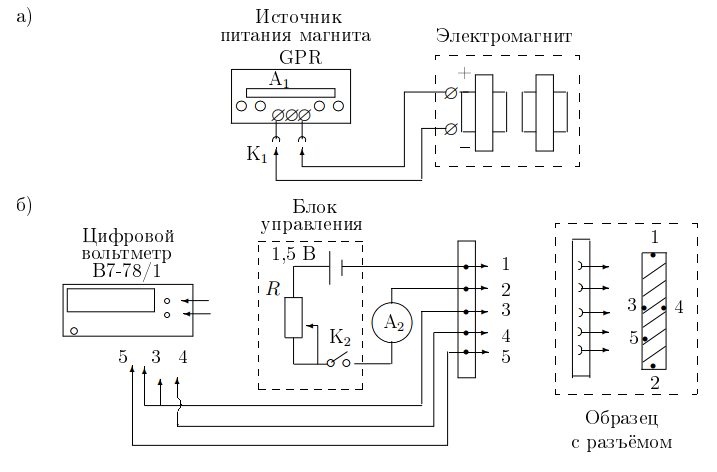
\includegraphics[height = 6cm, width = 12cm]{image1.png}
	\caption{Схема установки для исследования эффекта Холла в полупроводниках}
\end{figure}
\par
	В зазоре электромагнита создаётся постоянное магнитное поле, величину которого можно менять с помощью регуляторов источника питания электромагнита. Ток питания электромагнита измеряется амперметром источника питания $A_1$. Разъём $K_1$ позволяет менять направление тока в обмотках электромагнита.
\par
	Образец из легированного германия, смонтированный в специальном держателе, подключается к батарее. При замыкании ключа $K_2$ вдоль длинной стороны образца течёт ток, величина которого регулируется реостатом $R$ и измеряется миллиамперметром $A_2$. В образце с током, помещённом в зазор электромагнита, между контактами 3 и 4 возникает разность потенциалом $U_\text{34}$, которая измеряется с помощью цифрового вольтметра.
\par
	Контакты 3 и 4 вследствие неточности подпайки не всегда лежат на одной эквипотенциали, и тогда напряжение между ними связано не только с эффектом Холла, но и с омическим падением напряжения, вызванным протеканием основного тока через образец. Измеряемая разность потенциалов при одном направлении магнитного поля равна сумме ЭДС Холла и омического падения напряжения, а при другом их разности. В этом случае ЭДС Холла $\mathbb{E}_x$ может быть определено как половина алгебраической разности показаний вольтметра, полученных для двух противоположных направлений магнитного поля в зазоре.
\par
	Однако можно исключить влияние омического падения напряжения иначе, если при каждом токе через образец измерять напряжение между точками 3 и 4 в отсутствие магнитного поля. Тогда величина ЭДС Холла $\mathscr{E}_X = U_\text{34} + U_0$. При таком способе измерения нет необходимости проводить повторные измерения с противоложным направлением магнитного поля.
\par
	Измерив ток $I$ и напряжение $U_\text{35}$ между контактами 3 и 5 в отсутствие магнитного поля, можно, зная параметры образца, рассчитать проводимость материала образца:
\[
	\sigma = \frac{L_\text{35}}{a \cdot l} \, \frac{I}{U_\text{35}},
\]		 		 			
где $L_\text{35}$ --- расстояние между контактами 3 и 5, $a$ --- толщина образца, $l$ --- его ширина.
\section*{Ход работы}
\subsection*{Параметры установки}
	В данной экспериментальной установке:
	\begin{align*}
		a = 2.2 \, \text{мм} \\
		L_\text{35} = 3.0 \, \text{мм} \\
		l = 2.5 \, \text{мм} \\ 
	\end{align*}
\subsection*{Градуировка электромагнита}
	Проведём измерения магнитной индукции $B$ в зависимости от значения тока через электромагнит $I_m$ и построим график зависимости $B = f(I_m)$.
\begin{table}[h!]
	\centering
	\begin{tabular}{|c|c|c|c|c|c|c|c|c|c|c|}
	\hline
	$B$, мТл & 887 & 840 & 784 & 712 & 629 & 537 & 441 & 340 & 253 & 143 \\
	\hline
	$I$, А & 1.05 & 0.95 & 0.85 & 0.75 & 0.65 & 0.54 & 0.44 & 0.34 & 0.25 & 0.15 \\
	\hline
	\end{tabular}
\end{table}
\newpage
\begin{figure}[h!]
	\centering
	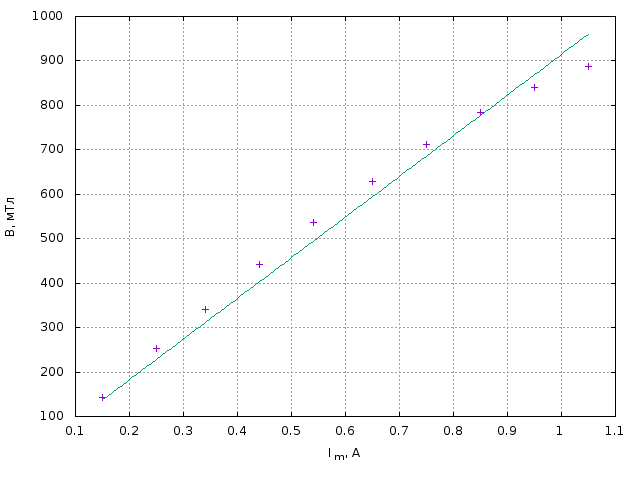
\includegraphics[height = 6.5cm, width = 12cm]{plot1.png}
	\caption{График зависимости $B = f(I_m)$}
\end{figure}
	Определив коэффициент наклона графика, получим, что:
\[
	B = 915 \cdot I \quad \left(\sigma_B = 2 \% \right), 
\]	
где $I$ измеряется в амперах, а значение $B$ получается в миллитеслах.	
\subsection*{Измерение ЭДС Холла}
\begin{enumerate}
	\item
		Проведём измерения ЭДС Холла при различных значениях тока через образец. Для этого 			вставим образец в зазор выключенного электромагнита и будем определять напряжение $U_0$ 		между холловскими контактами 3 и 4 для каждого значения тока через образец. Включив 			электромагнит, снимем зависимость напряжения $U_\text{34}$ от тока $I_m$ через обмотки 			магнита для каждого фиксированного тока через образец.
    \begin{table}[h!]
		\centering
		\begin{tabular}{|c|c|c|c|c|c|c|c|c|}
		\hline
			$\mathscr{E}_x$, мкВ & $-44$ & $-41$ & $-38$ & $-35$ & $-31$ & $-28$ & $-22$ & $-16$ \\
		\hline
			$I$, А & $1.19$ & $1.00$ & $0.9$ & $0.8$ & $0.7$ & $0.6$ & $0.5$ & $0.35$ \\
		\hline	
		\end{tabular}
		\caption{Таблица измерения $U_\text{34} = f(I_m)$ при $I = 0.25$ мА и $U_0 = -10 $ мкВ}
	\end{table}
	\begin{table}[h!]
		\centering
		\begin{tabular}{|c|c|c|c|c|c|c|c|c|}
		\hline
			$\mathscr{E}_x$, мкВ & $-71$ & $-65$ & $-59$ & $-50$ & $-41$ & $-35$ & $-23$ \\
		\hline
			$I$, А & $1.25$ & $1.05$ & $0.9$ & $0.75$ & $0.6$ & $0.5$ & $0.35$ \\
		\hline	
		\end{tabular}
		\caption{Таблица измерения $U_\text{34} = f(I_m)$ при $I = 0.4$ мА и $U_0 = -15 $ мкВ}
	\end{table}
	\begin{table}[h!]
		\centering
		\begin{tabular}{|c|c|c|c|c|c|c|c|c|}
		\hline
			$\mathscr{E}_x$, мкВ & $-89$ & $-82$ & $-74$ & $-63$ & $-52$ & $-43$ & $-29$ \\
		\hline
			$I$, А & $1.25$ & $1.05$ & $0.9$ & $0.75$ & $0.6$ & $0.5$ & $0.35$ \\
		\hline	
		\end{tabular}		
		\caption{Таблица измерения $U_\text{34} = f(I_m)$ при $I = 0.5$ мА и $U_0 = -19 $ мкВ}
	\end{table}
	\newpage
	\begin{table}[h!]
		\centering
		\begin{tabular}{|c|c|c|c|c|c|c|c|c|}
		\hline
			$\mathscr{E}_x$, мкВ & $-106$ & $-97$ & $-87$ & $-75$ & $-61$ & $-51$ & $-35$ \\
		\hline
			$I$, А & $1.25$ & $1.05$ & $0.9$ & $0.75$ & $0.6$ & $0.5$ & $0.35$ \\
		\hline	
		\end{tabular}
		\caption{Таблица измерения $U_\text{34} = f(I_m)$ при $I = 0.6$ мА и $U_0 = -22 $ мкВ}
	\end{table}
	\begin{table}[h!]
		\centering
		\begin{tabular}{|c|c|c|c|c|c|c|c|c|}
		\hline
			$\mathscr{E}_x$, мкВ & $-124$ & $-113$ & $-103$ & $-88$ & $-71$ & $-59$ & $-42$ \\
		\hline
			$I$, А & $1.25$ & $1.05$ & $0.9$ & $0.75$ & $0.6$ & $0.5$ & $0.35$\\
		\hline	
		\end{tabular}
		\caption{Таблица измерения $U_\text{34} = f(I_m)$ при $I = 0.7$ мА и $U_0 = -26$ мкВ}
	\end{table}
	\begin{table}[h!]
		\centering
		\begin{tabular}{|c|c|c|c|c|c|c|c|c|}
		\hline
			$\mathscr{E}_x$, мкВ & $-142$ & $-129$ & $-117$ & $-101$ & $-82$ & $-69$ & $-48$ \\
		\hline
			$I$, А & $1.25$ & $1.05$ & $0.9$ & $0.75$ & $0.6$ & $0.5$ & $0.35$\\
		\hline	
		\end{tabular}
		\caption{Таблица измерения $U_\text{34} = f(I_m)$ при $I = 0.8$ мА и $U_0 = -30 $ мкВ}
	\end{table}
	\begin{table}[h!]
		\centering
		\begin{tabular}{|c|c|c|c|c|c|c|c|c|}
		\hline
			$\mathscr{E}_x$, мкВ & $-163$ & $-146$ & $-132$ & $-114$ & $-92$ & $-77$ & $-53$\\
		\hline
			$I$, А & $1.25$ & $1.05$ & $0.9$ & $0.75$ & $0.6$ & $0.5$ & $0.35$\\
		\hline	
		\end{tabular}
		\caption{Таблица измерения $U_\text{34} = f(I_m)$ при $I = 0.9$ мА и $U_0 = -33 $ мкВ}
	\end{table}
	\begin{table}[h!]
		\centering
		\begin{tabular}{|c|c|c|c|c|c|c|c|c|}
		\hline
			$\mathscr{E}_x$, мкВ & $-178$ & $-163$ & $-147$ & $-127$ & $-103$ & $-87$ & $-59$ \\
		\hline
			$I$, А & $1.25$ & $1.05$ & $0.9$ & $0.75$ & $0.6$ & $0.5$ & $0.35$ \\
		\hline	
		\end{tabular}
		\caption{Таблица измерения $U_\text{34} = f(I_m)$ при $I = 1.0$ мА и $U_0 = -37 $ мкВ}
	\end{table}
\par
	Проведём измерения $U_\text{34} = f(I_m)$ при другом направлении магнитного поля (повернув образец на $180 \degree$ вокруг горизонтальной оси, проходящей вдоль ручки держателя).
	\begin{table}[h!]
		\centering
		\begin{tabular}{|c|c|c|c|c|c|c|c|c|}
		\hline
			$\mathscr{E}_x$, мкВ & $-178$ & $-163$ & $-147$ & $-126$ & $-104$ & $-86$ & $-61$ \\
		\hline
			$I$, А & $1.25$ & $1.05$ & $0.9$ & $0.75$ & $0.6$ & $0.5$ & $0.35$ \\
		\hline	
		\end{tabular}
		\caption{Таблица измерения $U_\text{34} = f(I_m)$ при $I = 1.0$ мА и $U_0 = -44 $ мкВ}
	\end{table}
\item
	Построим семейство характеристик $\mathscr{E}_x = f(B) $ при разных значениях тока $I$ через образец. Определим угловые коэффициенты $k(I) = \Delta \mathscr{E}_x / \Delta B$ полученных прямых.
	\newpage
	\begin{figure}[h!]
		\centering
		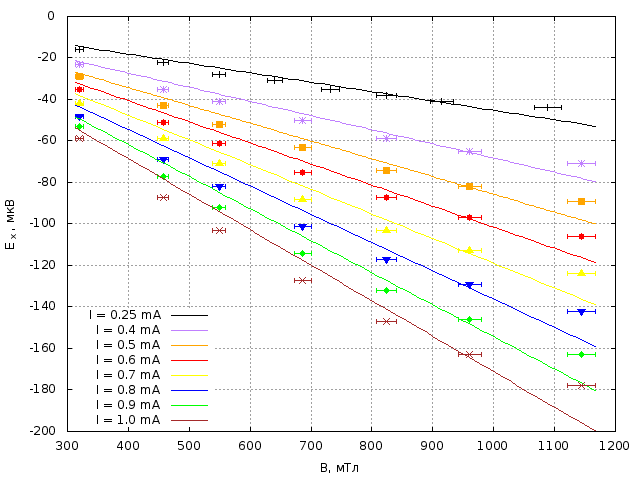
\includegraphics[height = 8cm, width = 15cm]{plot2.png}
		\caption{График зависимости $\mathscr{E}_x = f(B)$ при разных значениях тока $I$}
	\end{figure}
	\begin{table}[h!]
		\centering
		\begin{tabular}{|c|c|c|}
		\hline
			$k(I)$, мВ / Тл & $I$, мА & $\Delta_k$ \\
		\hline
			$-0.0452$ & $0.25$ & $0.0013$ \\
		\hline
			$-0.068$ & $0.4$ & $0.002$ \\
		\hline
			$-0.086$ & $0.5$ & $0.003$ \\
		\hline
			$-0.102$ & $0.6$ & $0.003$ \\
		\hline
			$-0.119$ & $0.7$ & $0.003$ \\
		\hline
			$-0.136$ & $0.8$ & $0.004$ \\
		\hline
			$-0.154$ & $0.9$ & $0.004$ \\
		\hline
			$-0.171$ & $1.0$ & $0.005$ \\							 	
		\hline
		\end{tabular}
	\end{table}	
	\item
		Построим график $k = f(I)$ и найдём коэффициент его наклона. Определим величину постоянной Холла $R_x$ как
	\[
		R_x = - \frac{\Delta k(I)}{\Delta I} \cdot a
	\]
		Далее рассчитаем концетрацию $n$ носителей тока в образце по формуле:
	\[
		n = \frac{1}{e \cdot R_x}
	\]			
	\newpage
	\begin{figure}[h!]
		\centering
		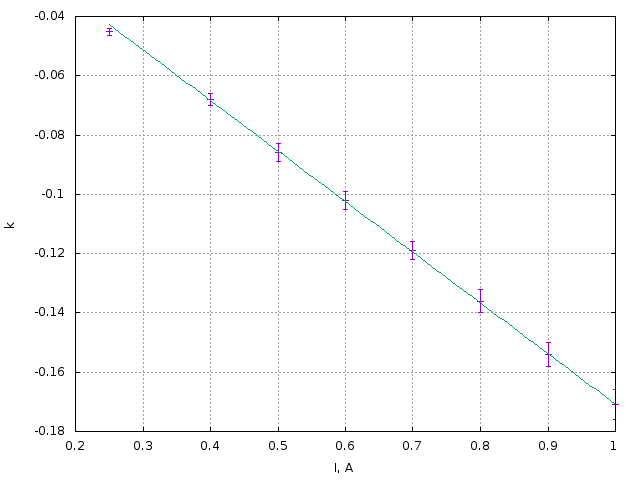
\includegraphics[height = 6cm, width = 12cm]{plot3.png}
		\caption{График зависимости $k = f(I)$}
	\end{figure}
	С помощью метода наименьших квадратов получим, что
	\[
		\frac{\Delta k(I)}{\Delta I} = - \left(170.8 \pm 0.5 \right) \cdot 10^{-3}\, \frac{\text{B}}{\text{Тл} \cdot \text{А}}
	\]
	Следовательно, 
	\[
		R_x = \left(357.6 \pm 1.2 \right) \cdot 10^{-6} \, \frac{{\text{м}}^3}{\text{Кл}} 
	\]
	Тогда концентрация носителей тока в образце
	\[
		n = \left(1.748 \pm 0.006 \right) \cdot 10^{22} \, \frac{1}{\text{м}^3}
	\]
\end{enumerate}
\subsection*{Определение характера проводимости}
	В данном случае проводимость дырочная. Иллюстрации приведены в приложении к отчёту.
\subsection*{Определение удельной проводимости}	
	При токе через образец $I = 1$ мА измерим падение напряжения $U_\text{35}$. Получим, что $U_\text{35} = 1.765$ мВ. Проводимость материала 
	\[
		\sigma  = \left(309.0 \pm 0.2 \right) \frac{1}{\text{Ом} \cdot \text{м}}.  
	\]
	Следовательно, подвижность носителей тока 
	\[
		b = \frac{\sigma}{e n} = \left(1104\pm 3\right) \, \frac{{\text{см}}^2}{\text{В} \cdot \text{с}}
	\]
\end{document}